\documentclass[11pt,a4paper]{article}

% Packages
\usepackage[T1]{fontenc}
\usepackage[utf8]{inputenc}
\usepackage{lmodern}
\usepackage[margin=2.2cm]{geometry}
\usepackage{graphicx}
\usepackage{xcolor}
\usepackage{hyperref}
\usepackage{booktabs}
\usepackage{longtable}
\usepackage{tabularx}
\usepackage{float}
\usepackage{parskip}
\usepackage{multicol}
\usepackage{fancyhdr}
\usepackage{titlesec}
\usepackage{tcolorbox}
\usepackage{enumitem}
\usepackage{microtype}
\usepackage{wrapfig}

% Brand Colors
\definecolor{topshopblack}{HTML}{000000}
\definecolor{thgblue}{HTML}{0033A0}
\definecolor{irisviolet}{HTML}{6C3BA1}
\definecolor{accentgold}{HTML}{C4A35A}
\definecolor{lightgrey}{HTML}{F5F5F5}
\definecolor{medgrey}{HTML}{666666}
\definecolor{darkgrey}{HTML}{333333}

% Hyperref config
\hypersetup{
    colorlinks=true,
    linkcolor=thgblue,
    urlcolor=irisviolet,
    citecolor=thgblue,
    pdftitle={IRIS World Record Attempt - Agentic Campaign Generation},
    pdfauthor={THG Ingenuity x IRIS},
}

% Header/Footer
\pagestyle{fancy}
\fancyhf{}
\fancyhead[L]{\small\textcolor{medgrey}{IRIS World Record Attempt}}
\fancyhead[R]{\small\textcolor{medgrey}{THG Ingenuity | Topshop SS26}}
\fancyfoot[C]{\small\textcolor{medgrey}{\thepage}}
\renewcommand{\headrulewidth}{0.4pt}
\renewcommand{\footrulewidth}{0pt}

% Section styling
\titleformat{\section}{\Large\bfseries\color{topshopblack}}{}{0em}{}[\titlerule]
\titleformat{\subsection}{\large\bfseries\color{darkgrey}}{}{0em}{}
\titleformat{\subsubsection}{\normalsize\bfseries\color{medgrey}}{}{0em}{}

% tcolorbox styles
\tcbset{
    voiceprompt/.style={
        colback=lightgrey,
        colframe=irisviolet,
        coltitle=white,
        fonttitle=\bfseries,
        left=6pt,
        right=6pt,
        top=4pt,
        bottom=4pt,
        boxrule=1pt,
        arc=2pt,
    },
    metricbox/.style={
        colback=lightgrey,
        colframe=thgblue,
        coltitle=white,
        fonttitle=\bfseries,
        left=6pt,
        right=6pt,
        top=4pt,
        bottom=4pt,
        boxrule=0.5pt,
        arc=2pt,
    }
}

% Graphics path
\graphicspath{{figures/}}

\begin{document}

% ============================================================
% TITLE PAGE
% ============================================================
\begin{titlepage}
\centering
\vspace*{2cm}

{\Huge\bfseries IRIS World Record Attempt}\\[0.5cm]
{\LARGE\textcolor{thgblue}{Agentic Campaign Generation}}\\[0.3cm]
{\Large\textcolor{medgrey}{Topshop SS26 --- Style Reimagined}}\\[2cm]

% Partner logos
\begin{minipage}{0.3\textwidth}
    \centering
    \includegraphics[height=1.5cm]{logo_topshop.png}
\end{minipage}\hfill
\begin{minipage}{0.3\textwidth}
    \centering
    \includegraphics[height=1.5cm]{logo_thg.png}
\end{minipage}\hfill
\begin{minipage}{0.3\textwidth}
    \centering
    \includegraphics[height=1.5cm]{logo_dreamlab.png}
\end{minipage}

\vspace{0.8cm}

{\large
\textcolor{irisviolet}{\textbf{THG Ingenuity}} $\times$ \textbf{IRIS Autonomous System}\\[0.3cm]
\textcolor{medgrey}{\textbf{DreamLab AI Consulting Ltd}}\\[0.3cm]
\textcolor{medgrey}{February 25, 2026}
}

\vfill

\begin{tcolorbox}[metricbox, title=Campaign Metrics at a Glance, width=0.85\textwidth]
\begin{center}
\begin{tabular}{lcl}
\textbf{Total Assets Generated} & \quad & \textbf{133} images and videos \\
\textbf{Wall-Clock Time} & \quad & \textbf{96 minutes} (first config to last asset) \\
\textbf{Active Generation Time} & \quad & \textbf{$\sim$64 minutes} \\
\textbf{Traditional Baseline} & \quad & 4 hours (expert operator) \\
\textbf{Speedup} & \quad & \textbf{8$\times$} (36 assets) to \textbf{14$\times$} (133 assets)\textsuperscript{*} \\
\textbf{Voice Prompts} & \quad & 21 (16 asset generation, 5 documentation/QA) \\
\textbf{Human Input Time} & \quad & $\sim$5 minutes total \\
\textbf{AI Engines Used} & \quad & 3 (Flux~2 Dev, Gemini~2.5 Flash, Veo~3.1) + PIL \\
\end{tabular}
\end{center}
\end{tcolorbox}

\vspace{1cm}
{\small\textcolor{medgrey}{Based on the THG Ingenuity ``Runway to the Future'' workflow,\\originally built in Freepik Spaces with a 4-hour build time\\and 15-minute per-asset generation cycle.}}

{\footnotesize\textcolor{medgrey}{\textsuperscript{*}Traditional estimates for $>$36 assets are linear extrapolations from the measured per-asset rate and may overestimate traditional times.}}
\end{titlepage}

% ============================================================
% TABLE OF CONTENTS
% ============================================================
\tableofcontents
\newpage

% ============================================================
% 1. EXECUTIVE SUMMARY
% ============================================================
\section{Executive Summary}

On February 25, 2026, the IRIS autonomous campaign generation system attempted to set a world record for AI-generated fashion advertising. Starting from a single four-panel garment photograph---Look~6 from the Topshop SS26 collection---an autonomous AI agent swarm produced 133 campaign assets in 96 minutes of wall-clock time (64 minutes of active generation).

Critically, this was achieved \textbf{from a standing start in 3 hours on-site at THG}---no pre-built workflows, no pre-existing assets, no creative brief. The human creative director \textbf{never opened a creative interface}. No GUI was used. No manual pipeline construction. No drag-and-drop workflow building. The operator spoke voice instructions; the AI agent swarm autonomously constructed every workflow from scratch---the multi-GPU pipeline configuration, ComfyUI workflow JSON files, API integrations, Nano Banana (a ComfyUI custom node wrapping Google's Gemini~2.5 Flash Image API) prompt engineering, Veo~3.1 video generation calls, programmatic compositing scripts, and quality assurance checks. Everything---the pipeline architecture, asset generation, error recovery, documentation, and this formal report---was produced within that 3-hour window using a mix of local GPU compute and cloud AI services, directed entirely by voice.

This work builds on a workflow pioneered by THG Ingenuity for the \textbf{Agentic Catwalk} event in February 2026. That original workflow, built manually within the Freepik Spaces visual interface by a skilled operator, required approximately 4 hours of expert setup time and produced assets at a rate of roughly 15 minutes per image. The IRIS system autonomously \textbf{generated all equivalent workflows from scratch}---with no human interaction with any creative tool, no manual node wiring, no parameter tuning---achieving:

\begin{itemize}[nosep]
    \item \textbf{8--14$\times$ speedup} over the traditional 4-hour expert pipeline (see caveats in Section~\ref{sec:timing})
    \item \textbf{133 assets} from 21 voice prompts (16 directing generation, 5 directing documentation and QA) totalling $\sim$5 minutes of human input
    \item \textbf{Peak generation rate} of 4.4 images/minute during parallel swarm execution
    \item \textbf{Zero manual Photoshop} --- all compositing, typography, and formatting automated
\end{itemize}

The dress---a cream sleeveless maxi with black ink botanical chrysanthemum illustrations on the bodice, thin vertical pinstripes on the A-line skirt, and thin chain link straps---remained the single constant element across all outputs, placed into environments spanning brutalist architecture, neon corridors, surreal smiley-filled voids, underwater dreamscapes, and more.

% ============================================================
% 2. TOPSHOP: RISE, FALL, AND RESURGENCE
% ============================================================
\section{Topshop: Rise, Fall, and Resurgence}

\subsection{The Rise of a British Icon (1964--2015)}

Topshop began in 1964 as a concession within Sheffield's Peter Robinson department store, quickly establishing itself as the destination for trend-driven, affordable fashion on the British high street. By the 1990s and 2000s, under the Arcadia Group and Sir Philip Green, Topshop had become a global fashion phenomenon.

The brand's Oxford Circus flagship store in London---spanning over 90,000 square feet across five floors---became one of the most visited fashion destinations in the world~\cite{wikipedia_topshop}. At its peak, Topshop operated over 500 stores across 37 countries. The brand's ``Topshop Unique'' runway shows during London Fashion Week cemented its position at the intersection of high street and high fashion.

Celebrity collaborations with Kate Moss (2007--2014) and Beyonc\'{e} generated massive cultural impact, while designer partnerships brought runway aesthetics to accessible price points.

\subsection{The Collapse (2018--2020)}

The decline was swift and multifactorial:
\begin{itemize}[nosep]
    \item Rising competition from fast-fashion e-commerce (ASOS, Boohoo, Shein)
    \item Shifting consumer behaviour away from high street retail
    \item Controversies surrounding Sir Philip Green
    \item The COVID-19 pandemic delivering the final blow
\end{itemize}

In November 2020, Arcadia Group entered administration, affecting approximately 13,000 jobs~\cite{itv2020arcadia}. Topshop's physical retail empire---once the envy of the fashion industry---ceased to exist.

\subsection{Acquisition and Digital Rebirth (2021--Present)}

In February 2021, ASOS acquired the Topshop, Topman, Miss Selfridge, and HIIT brands for \pounds 265 million~\cite{glc2021asos}, marking one of the most significant digital-first brand acquisitions in British fashion history. Under ASOS ownership, Topshop pivoted to an online-only model.

By 2024--2026, the brand has undergone a deliberate repositioning:
\begin{itemize}[nosep]
    \item New creative direction emphasising editorial quality
    \item Technology-forward campaigns leveraging AI and generative tools
    \item Partnership with THG Ingenuity for technology infrastructure
    \item Revival of the ``Style Reimagined'' brand messaging
\end{itemize}

\subsection{THG Ingenuity and the Technology Partnership}

THG (The Hut Group) operates one of the world's most advanced end-to-end e-commerce technology platforms through its \textbf{THG Ingenuity} division~\cite{thg_aboutus} (demerged into a standalone private company in January 2025~\cite{businesscloud2024demerger}). This proprietary platform provides:
\begin{itemize}[nosep]
    \item Global e-commerce infrastructure
    \item Content creation and management tools
    \item AI-powered product imagery and campaign generation
    \item Studio and production automation
\end{itemize}

THG Ingenuity's partnership with brands like Topshop represents the convergence of heritage fashion with cutting-edge technology---precisely the space where the Agentic Catwalk event and this world record attempt operate.

% ============================================================
% 3. THE AGENTIC CATWALK
% ============================================================
\section{The Agentic Catwalk Event}

\subsection{THG Ingenuity's Vision}

In February 2026, THG Ingenuity staged \textbf{``Runway to the Future''}---the world's first AI-driven shoppable catwalk~\cite{thg2025catwalk}, certified by the WRCA (World Record Certification Agency)~\cite{wrca}. Held at THG Studios, Manchester on 26~February 2026 with headline sponsor PayPal and technology partner Google Cloud~\cite{rtih2025catwalk}, the event demonstrated how autonomous AI systems could generate complete fashion advertising campaigns. The event showcased a workflow built within \textbf{Freepik Spaces}, an AI image generation platform~\cite{businesswire2025freepik}, that could produce professional campaign assets from garment photographs.

The original THG workflow characteristics:
\begin{itemize}[nosep]
    \item \textbf{Build time:} Approximately 4 hours for an expert to construct the pipeline
    \item \textbf{Generation rate:} $\sim$15 minutes per asset through the pipeline
    \item \textbf{Platform:} Freepik Spaces (cloud-based AI image generation)
    \item \textbf{Output:} Fashion campaign images suitable for e-commerce and social media
\end{itemize}

\subsection{From Freepik Spaces to IRIS: No Creative Interface Required}

The critical distinction between the THG baseline and the IRIS approach is not merely speed---it is the \textbf{complete elimination of the creative interface from the operator's workflow}. The THG pipeline requires an expert to manually construct node-based workflows in Freepik Spaces, configure each generation step, review and iterate through a GUI, and manually export results. IRIS replaces this entire interaction model: the human speaks, and autonomous AI agents handle every technical step:

\begin{enumerate}[nosep]
    \item Interpret natural language voice instructions into concrete technical tasks
    \item \textbf{Generate all workflows and pipeline configurations from scratch}---no templates, no pre-built nodes
    \item Self-organise into specialised agent swarms with appropriate tool selection
    \item Select and orchestrate multiple AI generation engines (local GPU + cloud APIs)
    \item Write and execute Python scripts, ComfyUI JSON workflows, and API calls autonomously
    \item Perform quality assurance, detect errors (e.g.\ garment fidelity, text misspelling), and self-correct
    \item Handle iteration, retry logic, and creative expansion without human intervention
\end{enumerate}

At no point during the 3-hour session did the human operator open ComfyUI, Freepik Spaces, Photoshop, or any other creative application. The three ComfyUI workflow files in this repository (\texttt{flux2-multigpu-campaign.json}, \texttt{nano-banana-garment-reskin.json}, \texttt{nano-banana-repose.json}) were \textbf{written entirely by the AI agents}---they exist as documentation of what the system built, not as tools the human used.

% ============================================================
% 4. THE IRIS SYSTEM
% ============================================================
\section{The IRIS System}

\subsection{Architecture Overview}

IRIS (\textbf{I}ntelligent \textbf{R}eal-time \textbf{I}ntegrated \textbf{S}tudio) is a voice-controlled AI system developed by \textbf{DreamLab AI Consulting Ltd} that works alongside creative teams rather than replacing them. Built on \textbf{VisionFlow}---an open-source GPU-accelerated knowledge graph engine (168,000 lines of Rust, MPL-2.0 licensed)---IRIS combines neuro-symbolic AI reasoning with autonomous agent orchestration for creative production workflows.

\subsubsection{The UKRI Agentic AI Pioneers Prize}

This world record attempt forms part of the development phase for the \textbf{UKRI Agentic AI Pioneers Prize}, a programme funded by Innovate UK. The project is a three-party consortium:

\begin{itemize}[nosep]
    \item \textbf{DreamLab AI Consulting Ltd} (Lead): Platform development, agent architecture, OWL~2 ontology engineering
    \item \textbf{THG Ingenuity} (Partner): Creative studio environment, brand workflows, commercial route-to-market
    \item \textbf{University of Salford} (Collaborator): Creative industries research, user evaluation, catwalk co-production
\end{itemize}

\subsubsection{Technology Readiness Level Progression}

The fashion catwalk event on 25--26 February 2026 at THG Studios, Manchester represents a critical TRL validation milestone. The system has progressed from \textbf{TRL~4} (component validation) through \textbf{TRL~5} (validation within THG's creative production context) to \textbf{TRL~6} (full system demonstration in a relevant operational environment). This world record attempt stress-tests the complete pipeline---from voice brief through agent-driven asset generation---in a live production setting.

\subsubsection{The VisionFlow Platform}

The IRIS screenshots below show the VisionFlow web interface---the platform on which IRIS is built. These are live captures from the system during the world record attempt session.

\begin{figure}[H]
\centering
\begin{minipage}{0.48\textwidth}
    \centering
    \includegraphics[width=\textwidth]{Screenshot_20260225_124427.png}
    \caption*{\small VisionFlow Control Centre: Spawn Hive Mind dialog with mesh topology, agent type selection, and the repose task instruction. Left panel shows 3D knowledge graph controls with 147 nodes and GPU instancing enabled.}
\end{minipage}\hfill
\begin{minipage}{0.48\textwidth}
    \centering
    \includegraphics[width=\textwidth]{Screenshot_20260225_124530.png}
    \caption*{\small VisionFlow 3D knowledge graph: GPU-accelerated force-directed layout showing clustered ontology nodes. Each cluster represents a semantic domain within the fashion ontology, rendered at 60~FPS via 100+ CUDA kernels.}
\end{minipage}
\caption{The IRIS/VisionFlow web interface---a 3D immersive knowledge graph with voice-controlled agent orchestration. The Hive Mind dialog (left) shows how agents are spawned with natural language task descriptions; the graph view (right) shows the OWL~2 ontology structure.}
\label{fig:iris_interface}
\end{figure}

\begin{figure}[H]
\centering
\begin{minipage}{0.48\textwidth}
    \centering
    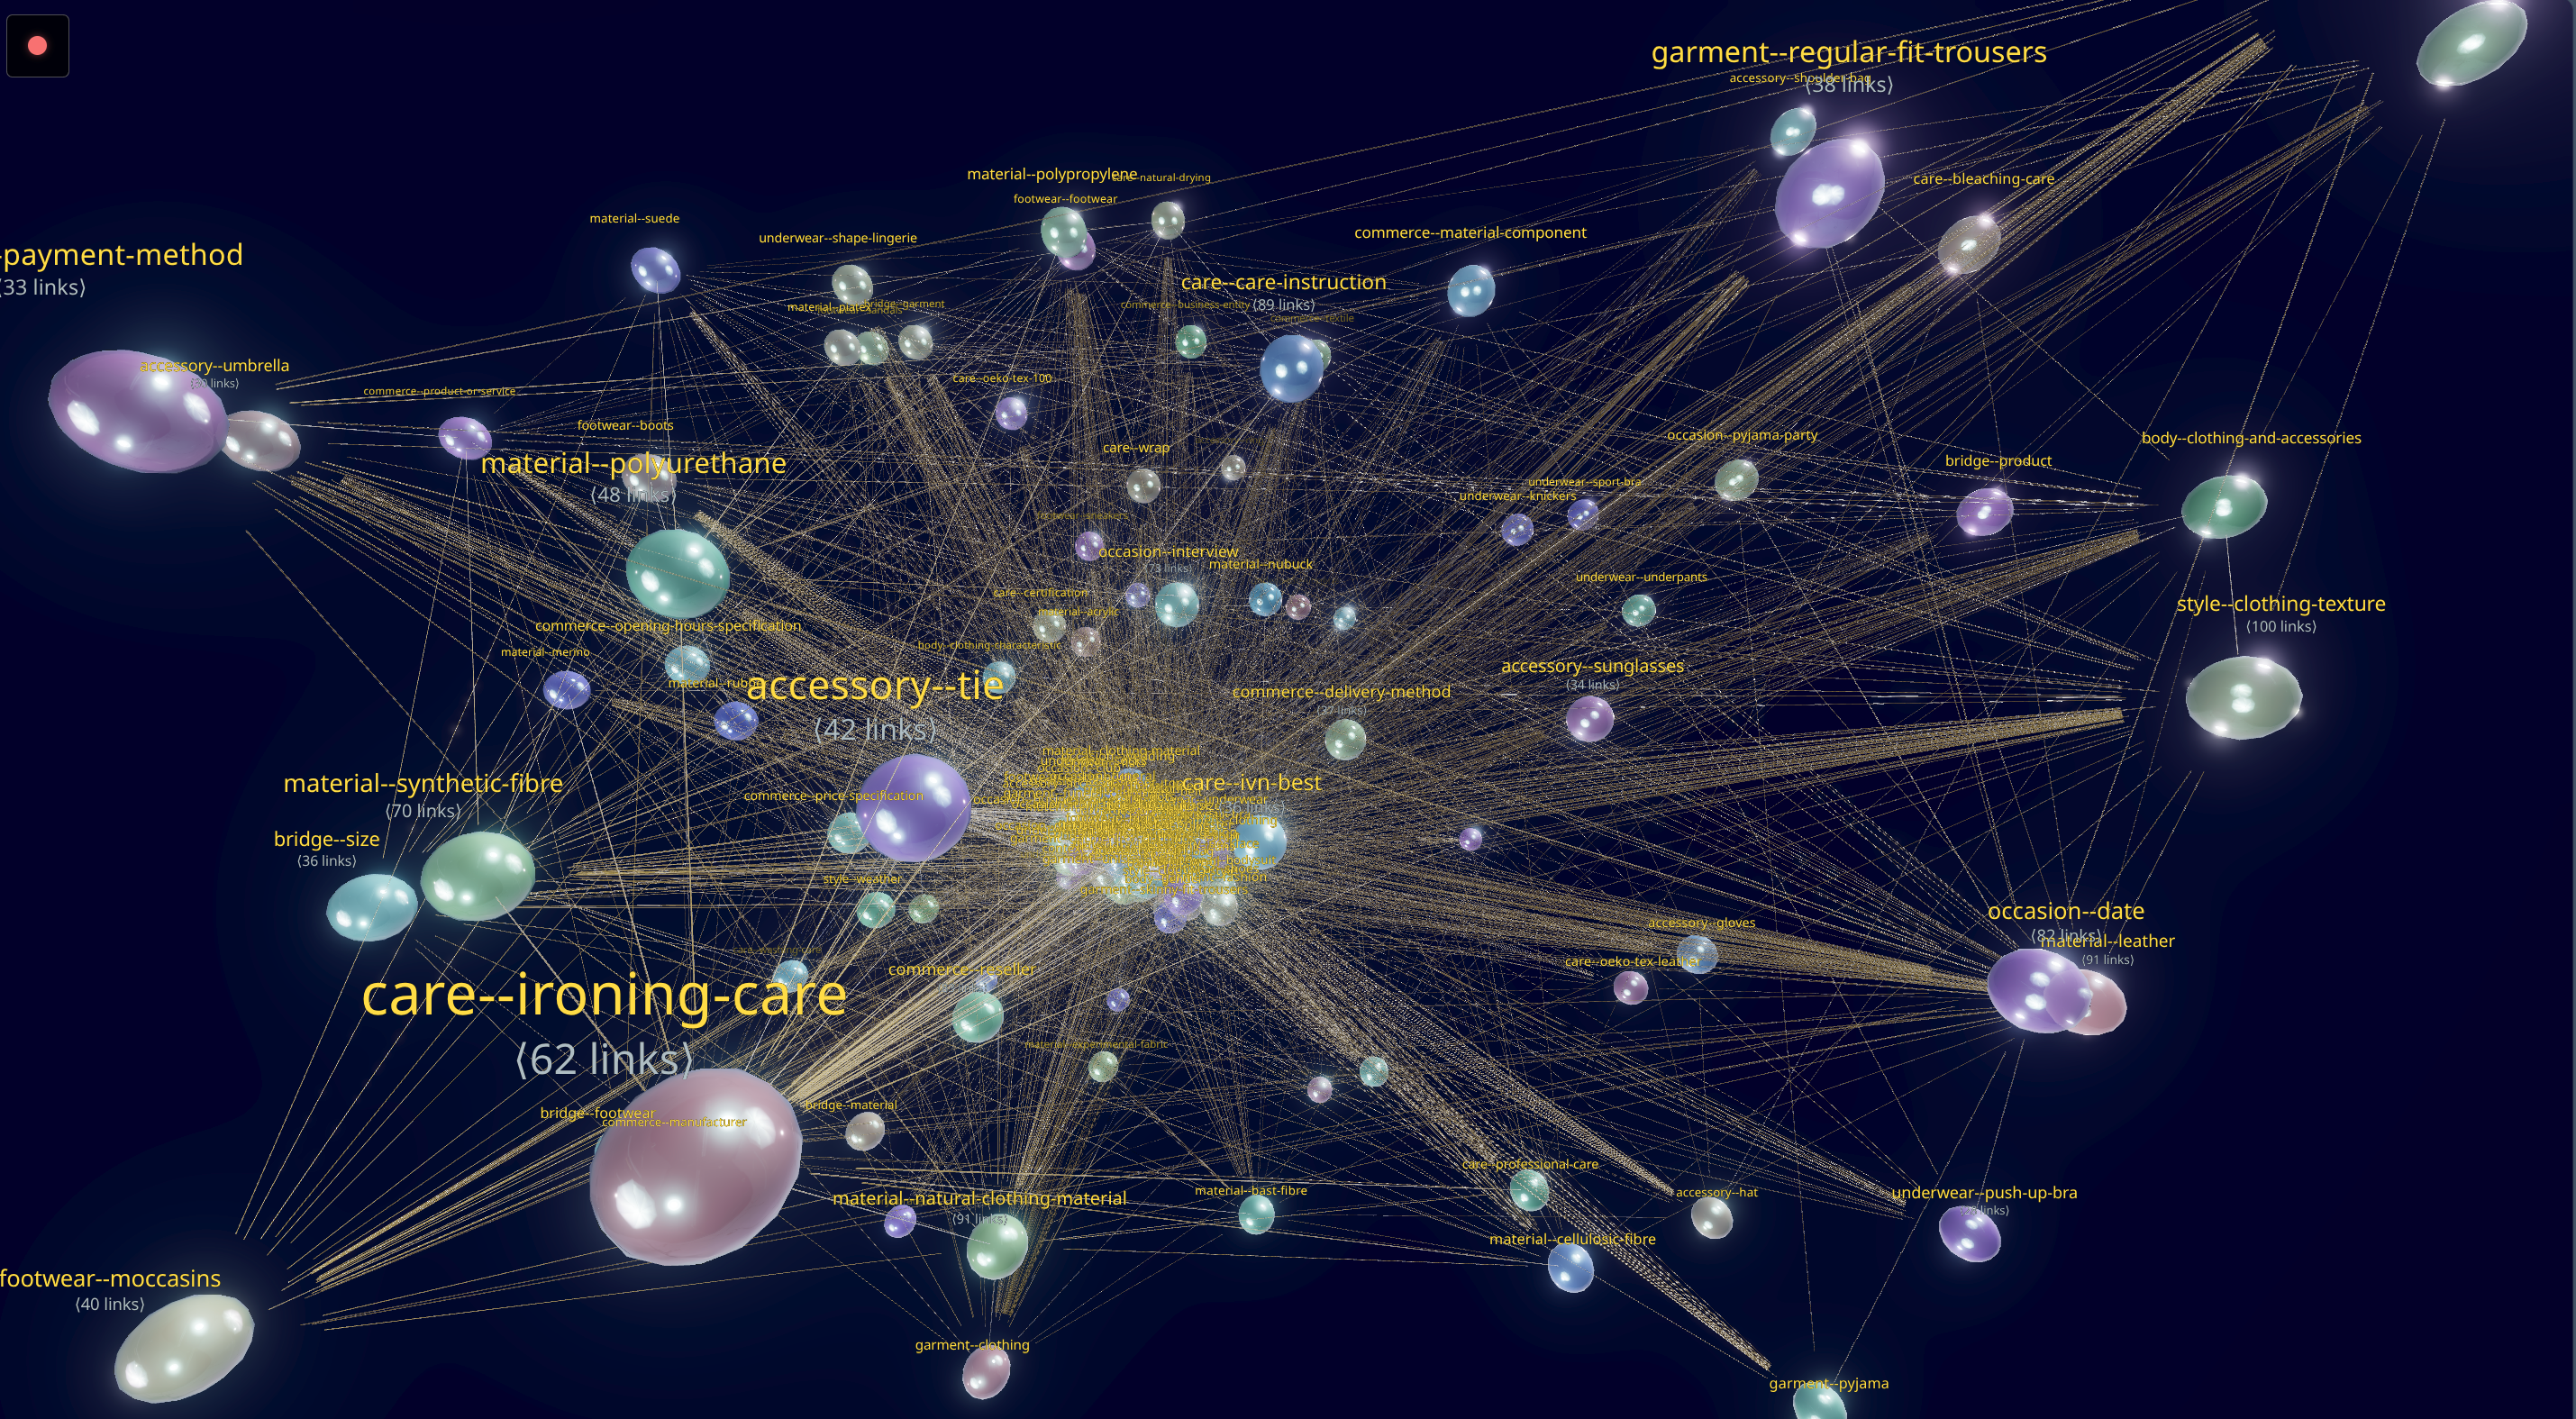
\includegraphics[width=\textwidth]{Screenshot_20260225_124750.png}
    \caption*{\small Fashion ontology detail: ``care--ironing-care'' (62 links), ``accessory--tie'' (42 links), ``garment--regular-fit-trousers'', ``material--polyurethane'', ``footwear--moccasins'', ``style--clothing-texture''. Each node represents a semantic concept in the OWL~2 ontology.}
\end{minipage}\hfill
\begin{minipage}{0.48\textwidth}
    \centering
    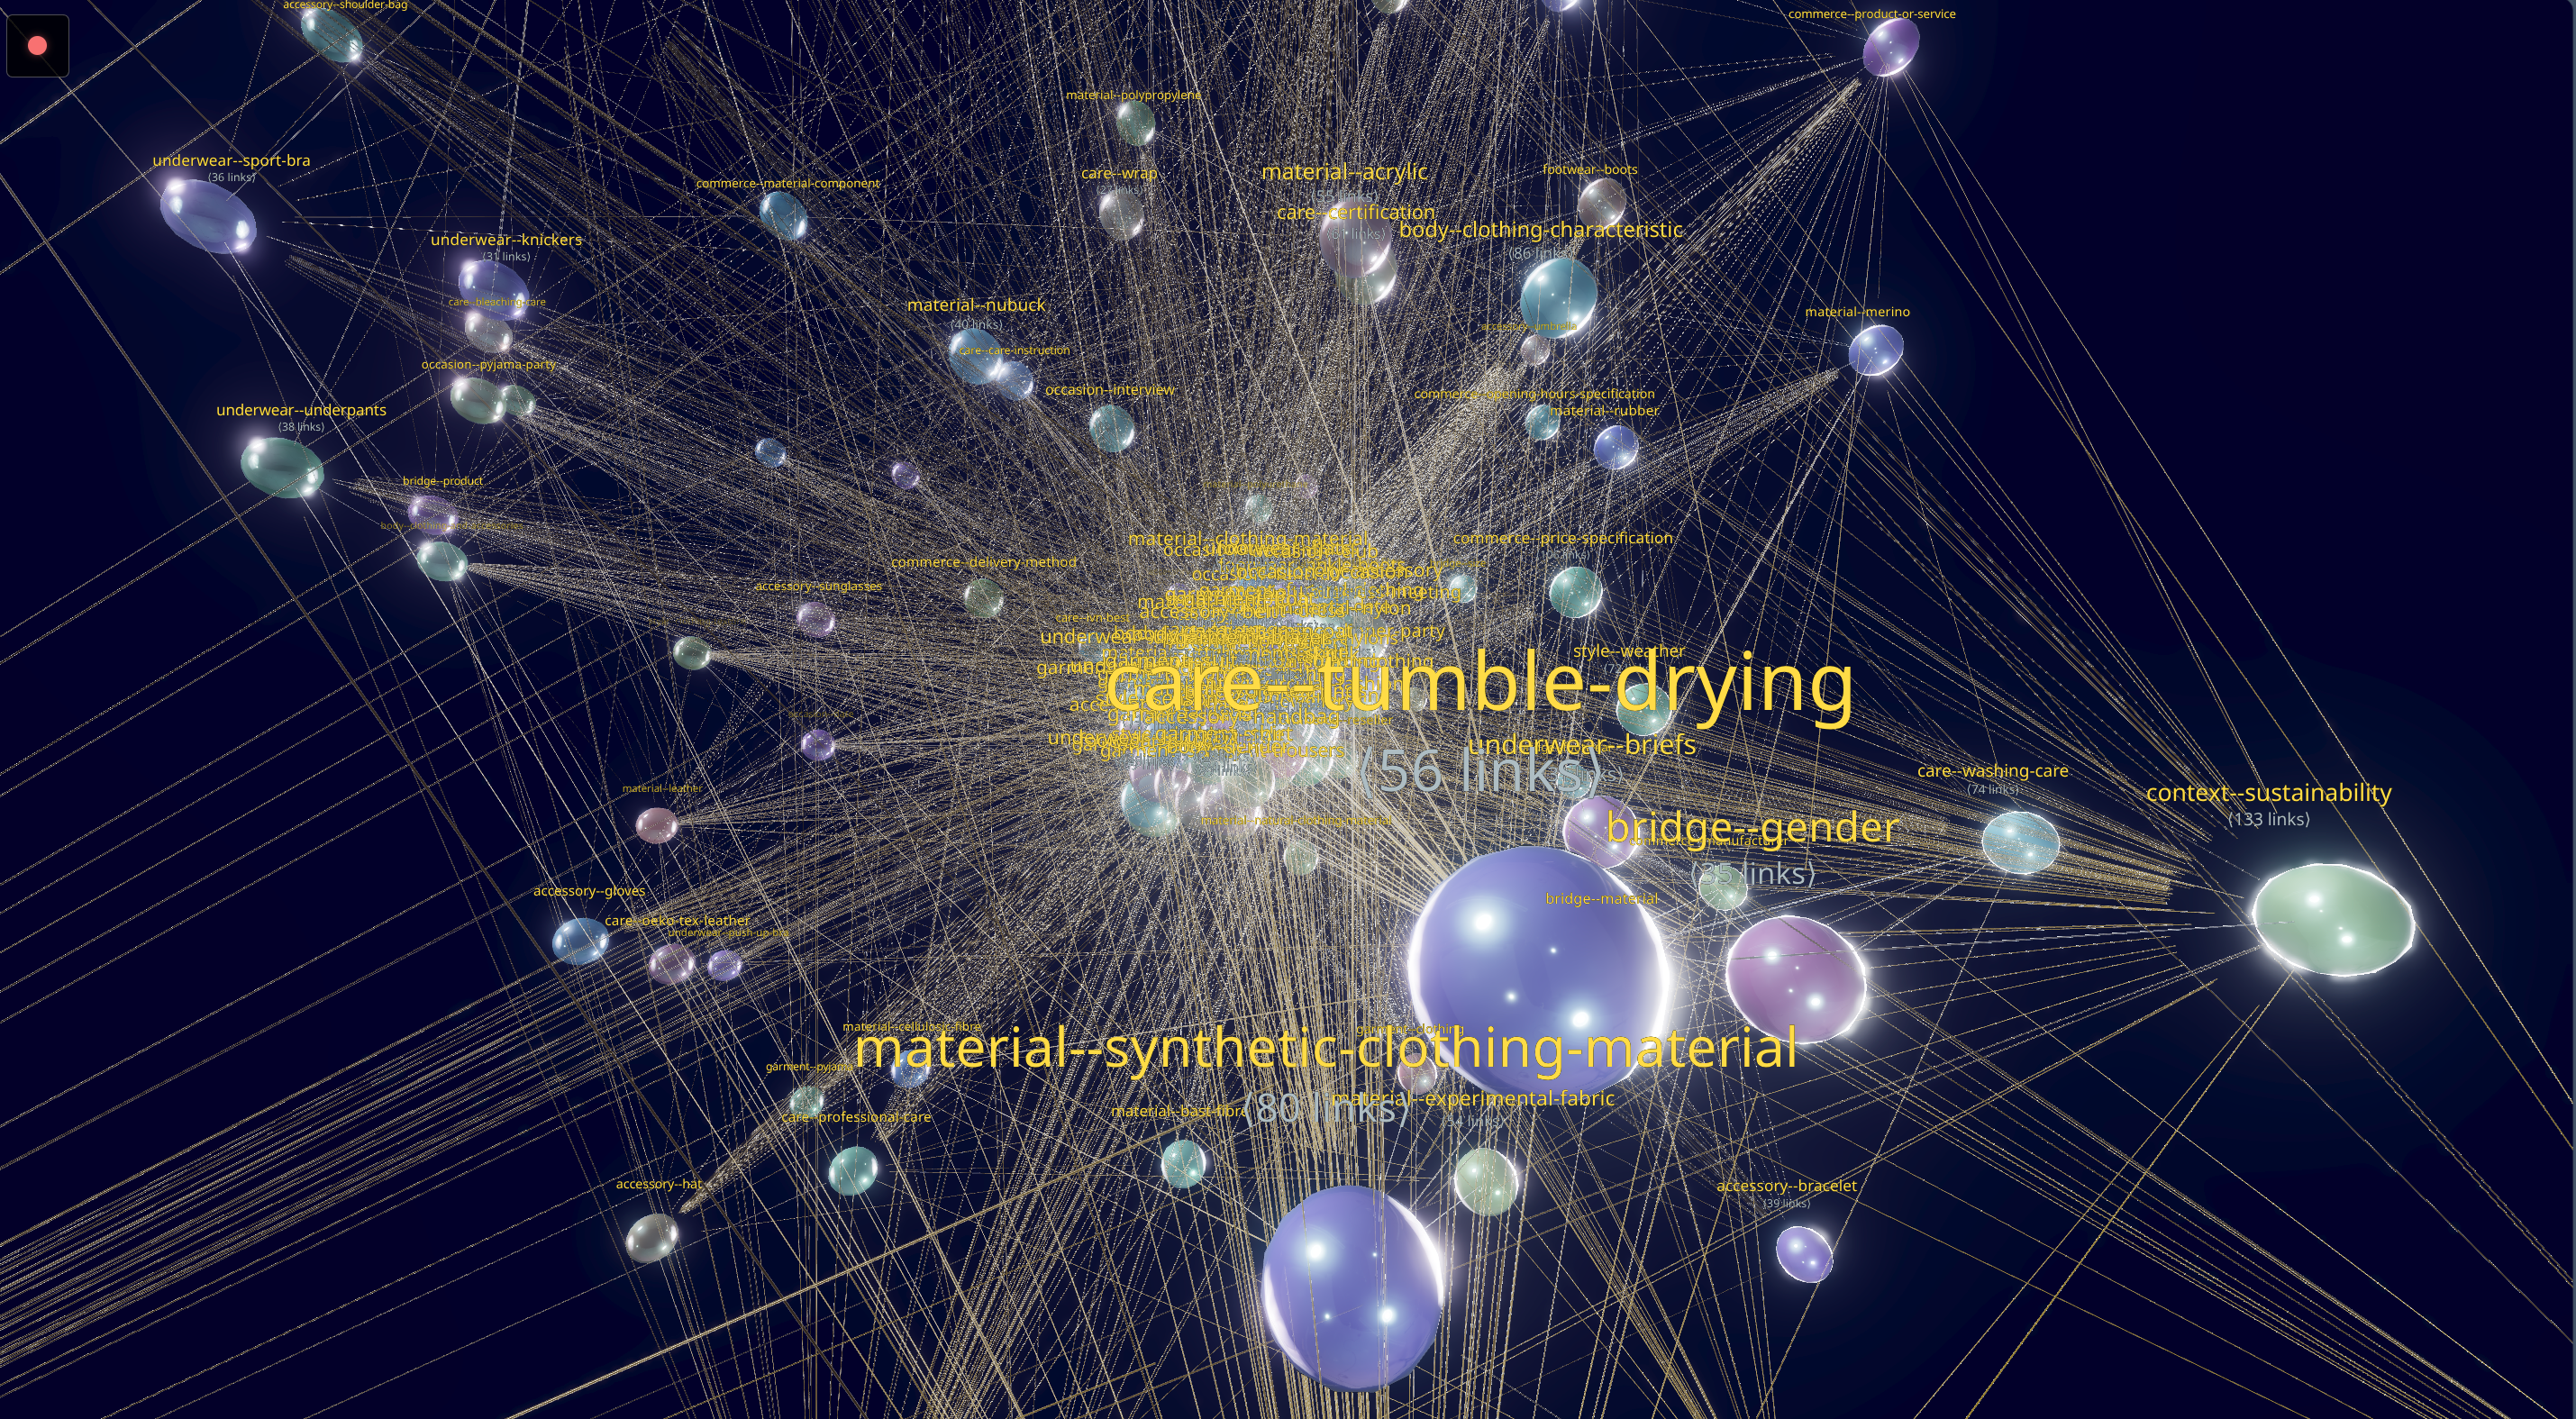
\includegraphics[width=\textwidth]{Screenshot_20260225_124904.png}
    \caption*{\small Dense ontology cluster: ``care--tumble-drying'' (56 links), ``material--synthetic-clothing-material'' (80 links), ``bridge--gender'', ``context--sustainability''. These relationships enable agents to reason about garment properties and care instructions.}
\end{minipage}
\caption{VisionFlow fashion knowledge graph close-ups showing OWL~2 ontology nodes with link counts. This is the structured, searchable knowledge layer that distinguishes IRIS from conventional AI creative tools---every creative decision is grounded in formal semantic relationships.}
\label{fig:iris_ontology}
\end{figure}

\subsubsection{Core Architecture}

IRIS implements a five-layer architecture: Presentation (React~19 + Three.js, WebXR), Compute (Rust/Actix-web, 100+ CUDA kernels), Knowledge (Neo4j + PostgreSQL + Qdrant unified under OWL~2 semantics), Agent (101 MCP skills via Claude-Flow coordinator), and Generative (containerised ComfyUI on local GPU). The core innovation is neuro-symbolic: agents reason over a formal OWL~2 ontology \emph{before} execution, rejecting semantically invalid proposals at the validation gate.

Three features distinguish IRIS: all generation runs on the studio's own hardware (IP sovereignty), creative workflows are captured as structured searchable knowledge (not unstructured files), and a human approves every client-facing output.

\begin{tcolorbox}[metricbox, title=IRIS System Architecture --- World Record Configuration]
\begin{itemize}[nosep]
    \item \textbf{Orchestration:} Claude Flow v3 Hierarchical Swarm
    \item \textbf{Local GPU:} 2$\times$ NVIDIA RTX 6000 Ada (48GB VRAM each)
    \item \textbf{Local Engine:} Flux 2 Dev FP8 via ComfyUI Multi-GPU
    \item \textbf{Cloud Engines:} Gemini 2.5 Flash Image (Nano Banana), Veo 3.1
    \item \textbf{Compositing:} PIL/Pillow programmatic rendering
    \item \textbf{Input Method:} Voice-captured natural language prompts
    \item \textbf{Max Parallel Agents:} 5 simultaneous (up to 50+ supported)
    \item \textbf{Platform:} VisionFlow (168K LoC Rust, MPL-2.0)
\end{itemize}
\end{tcolorbox}

\subsubsection{Voice-Captured Prompt Interface}

A critical distinction of the IRIS system is that all operator instructions were \textbf{voice-captured}---spoken naturally by the human creative director and transcribed into the system. This is not CLI input or typed commands; it represents the nominal operating mode for IRIS, where the creative director provides high-level artistic direction verbally, and the AI swarm handles all technical execution.

This voice-first approach means:
\begin{itemize}[nosep]
    \item Instructions are conversational and high-level, not technical
    \item The operator never writes code, API calls, or configuration files
    \item \textbf{The operator never opens a creative interface}---no ComfyUI, no Freepik Spaces, no Photoshop
    \item All workflows, scripts, and pipeline configurations are generated from scratch by the agents
    \item Each prompt averages $\sim$2 sentences of natural language
    \item The system interprets intent and autonomously determines implementation
\end{itemize}

\subsection{Multi-GPU Pipeline}

The local generation pipeline distributes Flux 2 Dev across dual RTX 6000 Ada GPUs:

\begin{table}[H]
\centering
\begin{tabular}{lll}
\toprule
\textbf{GPU} & \textbf{Component} & \textbf{VRAM} \\
\midrule
cuda:0 & Flux 2 Dev UNet (fp8mixed) & $\sim$38 GB \\
cuda:1 & Mistral 3 Small CLIP (fp8) + Flux 2 VAE & $\sim$19 GB \\
\bottomrule
\end{tabular}
\caption{Multi-GPU VRAM distribution via ComfyUI-MultiGPU custom nodes}
\end{table}

\subsection{Agent Swarm Composition}

The IRIS system deployed agents in three waves:

\textbf{Wave 1 --- Core Pipeline (4 agents):}
\begin{itemize}[nosep]
    \item \textbf{Creative Director:} Typography research, shot concepts, prompt library
    \item \textbf{Pipeline Executor:} 4-phase generation across 3 engines (142+ tool calls)
    \item \textbf{Brand Guardian:} Autonomous QA evaluation against brand criteria
    \item \textbf{Workflow Researcher:} API documentation and workflow guides
\end{itemize}

\textbf{Wave 2 --- Scene Riffs (5 agents):}
\begin{itemize}[nosep]
    \item \textbf{Scene Cleaner:} Remove mannequins from reference scenes, preserve environments
    \item \textbf{Direct Composite:} Place dress into scene environments (9 images)
    \item \textbf{Creative Riff:} Surreal editorial variations (10 images)
    \item \textbf{Expanded Riffs:} High-concept diverse variations (15 images)
    \item \textbf{Flux 2 Local:} GPU-rendered editorial scenes (8 images)
\end{itemize}

\textbf{Wave 3 --- Mannequin Repose (3 agents + 1 research):}
\begin{itemize}[nosep]
    \item \textbf{IRIS PDF Research:} Extract TRL/system context from 6 appendix documents
    \item \textbf{Repose Batch 1:} Images 1--10, alternating pose 24/26 (10 images)
    \item \textbf{Repose Batch 2:} Images 11--23, skipping ref 24 (13 images)
    \item \textbf{Repose Batch 3:} Images 25, 27--30, skipping ref 26 (5 images)
\end{itemize}

% ============================================================
% 5. THE GARMENT
% ============================================================
\section{The Garment: Topshop SS26 Look 6}

\begin{wrapfigure}{r}{0.3\textwidth}
    \centering
    \includegraphics[width=0.28\textwidth]{garment_reference.jpg}
    \caption{Garment reference: Look 6 front panel. The cream sleeveless maxi with botanical ink bodice, thin vertical pinstripes, and chain link straps.}
    \label{fig:garment}
\end{wrapfigure}

The entire campaign was generated from a single four-panel garment photograph showing front, right side, back, and left side views of \textbf{Look 6} from the Topshop SS26 collection.

\textbf{Garment details:}
\begin{itemize}[nosep]
    \item Cream/warm beige sleeveless maxi dress
    \item Delicate black ink botanical illustrations on the bodice: chrysanthemum flowers, bird silhouettes, flowing stems
    \item Thin vertical pinstripes on the flowing A-line skirt
    \item Thin chain link straps
    \item Natural, warm fabric tone
\end{itemize}

The four-panel composite was programmatically cropped into individual panels, with the front panel serving as the primary reference for all generation passes. The bottom 8\% of each panel was removed to exclude garment labels.

This single garment photograph served as the \textbf{sole creative input}. Every scene, environment, lighting condition, pose, and editorial concept was generated by the IRIS system from voice prompts alone.

\vspace{0.5cm}

% ============================================================
% 6. VOICE PROMPTS --- COMPLETE RECORD
% ============================================================
\section{Voice Prompts --- Complete Record}

All creative direction was provided as \textbf{voice-captured natural language prompts}. The operator spoke these instructions naturally; they were not typed CLI commands. This is the nominal input method for the IRIS system---a human creative director providing high-level artistic direction while the autonomous swarm handles all technical execution.

\begin{tcolorbox}[voiceprompt, title=Voice Prompt 1: Campaign Launch]
\small\itshape
``Generate a complete Topshop SS26 advertising campaign from a single garment photograph. Use Flux 2 Dev for base generation, Nano Banana for refinement, programmatic text for compositing, and Veo 3.1 for animation. Deploy as a Claude Flow v3 hierarchical swarm with Creative Director, Pipeline Executor, Brand Guardian, and Workflow Researcher agents.''
\end{tcolorbox}
\textbf{Result:} 4-agent swarm launched. 36 deliverables produced across 4 pipeline phases in 30 minutes.

\begin{tcolorbox}[voiceprompt, title=Voice Prompt 2: Garment Fidelity Correction]
\small\itshape
``Great work, we have not followed the EXACT garment from the ingest image though. Nano Banana can accomplish the reskinning.''
\end{tcolorbox}
\textbf{Result:} Identified bold diagonal stripes vs.\ actual thin vertical pinstripes. Triggered garment reskinning phase.

\begin{tcolorbox}[voiceprompt, title=Voice Prompt 3: ComfyUI Workflow Direction]
\small\itshape
``You can send the image to Nano Banana as a reference via the ComfyUI workflow.''
\end{tcolorbox}
\textbf{Result:} Created loadable JSON workflow using GeminiImageNode + ImageBatch approach.

\begin{tcolorbox}[voiceprompt, title=Voice Prompt 4: Continuous Delivery]
\small\itshape
``Commit and push when you get new results that look good.''
\end{tcolorbox}
\textbf{Result:} Continuous delivery pattern established. 30 reskinned assets pushed.

\begin{tcolorbox}[voiceprompt, title=Voice Prompt 5: Documentation and Workflows]
\small\itshape
``Also create a conventional JSON ComfyUI workflow that I can load into the UI on my ComfyUI and push that. Use a document agent and your memory to document the whole process we have undertaken.''
\end{tcolorbox}
\textbf{Result:} Two ComfyUI workflows + 1,496-line process documentation created and pushed.

\begin{tcolorbox}[voiceprompt, title=Voice Prompt 6: Scene Riffs Creative Brief]
\small\itshape
``I have added a directory with scene ideas as images, to GitHub. Pull down and figure out the best way of placing our mannequin and the reference dress into the new scenes, or variations of them. Keep the floating smiley faces. You can do a multi-step workflow, removing the current subjects from the images to create a cleaner pipeline for the image manipulation. Riff on the ideas, using your intelligence, Flux 2 image to image, Nano Banana, until you have an incredible set of composite ideas with the dress as the only consistent factor. Play with the ideas and be creative. When you have some incredible images continue with the branding and video creation.''
\end{tcolorbox}
\textbf{Result:} 5-agent parallel swarm launched targeting 45 new images across surreal, editorial, cyberpunk, nature, pop-art, and architectural concepts.

\begin{tcolorbox}[voiceprompt, title=Voice Prompt 7: Parallel Execution]
\small\itshape
``You can work in parallel with your swarm.''
\end{tcolorbox}
\textbf{Result:} Confirmed parallel agent execution across all 5 agents.

\begin{tcolorbox}[voiceprompt, title=Voice Prompt 8: Push Documentation]
\small\itshape
``Document all this. Do a push.''
\end{tcolorbox}
\textbf{Result:} Phase 5 documentation added and committed.

\begin{tcolorbox}[voiceprompt, title=Voice Prompt 9: Local GPU Clarification]
\small\itshape
``We don't have FluxKontext API keys, instead we have the local Flux 2 Dev model.''
\end{tcolorbox}
\textbf{Result:} Pipeline confirmed: local Flux 2 Dev + cloud Nano Banana API only.

\begin{tcolorbox}[voiceprompt, title=Voice Prompt 10: Expand Creative Diversity]
\small\itshape
``Increase the diversity of concepts and work within and without the new scene images, riffing and expanding but keeping a core.''
\end{tcolorbox}
\textbf{Result:} Two additional agents launched: 15 expanded concept variations + 8 Flux 2 local renders.

\begin{tcolorbox}[voiceprompt, title=Voice Prompt 11: Metrics and Traditional Comparison]
\small\itshape
``Add all of the prompts I have given you to the records of what we did. Label them as voice prompts. Measure the asset creation rate. Explain the time this workflow took to create using timestamp analysis. The traditional workflow we based all this on was around 4 hours for an expert with 15 minutes per generation on the pipeline.''
\end{tcolorbox}
\textbf{Result:} Comprehensive timing analysis document with voice prompt record created.

\begin{tcolorbox}[voiceprompt, title=Voice Prompt 12: Formal Report with Research]
\small\itshape
``Use Perplexity research agents to create a narrative about Topshop, its market crash and resurgence. When you have the history and vibe of Topshop you should look up the Agentic Catwalk event by THG Ingenuity in Feb 2026 and build information on that. This work is based on a THG workflow built in Freepik Spaces, which took 4 hours to build and has a 15 minute run per asset. The world record attempt today has used our system called IRIS to agentically recreate the workflow, and create assets for the world record event. Use the notes you have about the development we have undertaken, and Topshop and THG branding downloaded from the web. Create a thorough PDF document report on this using your LaTeX skill, compile, debug, and push to the GitHub.''
\end{tcolorbox}
\textbf{Result:} Research agents deployed. This document.

\begin{tcolorbox}[voiceprompt, title=Voice Prompt 13: Include All Prompts]
\small\itshape
``Include all the prompts, including this one.''
\end{tcolorbox}
\textbf{Result:} All voice prompts recorded in this section.

\begin{tcolorbox}[voiceprompt, title=Voice Prompt 14: Inline Images]
\small\itshape
``Build all of the images into the document inline, including explanation of their role in the development of the final assets.''
\end{tcolorbox}
\textbf{Result:} 46 figures prepared and embedded throughout this document.

\begin{tcolorbox}[voiceprompt, title=Voice Prompt 15: Voice Capture Clarification]
\small\itshape
``Explain that the prompts were voice captured from the user, not CLI input here, which is the nominal approach for the IRIS system.''
\end{tcolorbox}
\textbf{Result:} Voice-capture methodology documented throughout.

\begin{tcolorbox}[voiceprompt, title=Voice Prompt 16: IRIS Context and Mannequin Repose Task]
\small\itshape
``Two new tasks for the swarm. I have added much more context on IRIS. I am demonstrating progression from TRL4 to TRL6 for this THG and Topshop catwalk event. All the context for my IRIS system including the correct name and my interest is in those PDFs which you should research. Use that knowledge to add to the report without being overwhelming as this report targets multi audiences. Also, there's a new image task. We have a new folder called task-two-repose. We need to use our tooling to repose each image to match the stance of either of the new images 24 or 26, keeping all else the same for the images. This is likely a Nano Banana task and should be done at 2K resolution in the appropriate aspect for the task. When you have validated those results you can push. Update all the documentation accordingly for this new evolved context and additional work, this still fits in the original 3 hours.''
\end{tcolorbox}
\textbf{Result:} IRIS PDF research agent deployed across 6 appendix documents. 3 parallel repose agents launched, producing 28 reposed mannequin images. Report updated with IRIS/TRL context. All documentation updated.

\begin{tcolorbox}[voiceprompt, title=Voice Prompt 17: IRIS Screenshots and Full QA Pass]
\small\itshape
``I added some screenshots from the IRIS web interface into the figures directory on GitHub, pull and integrate into the report. Ensure the report is fully up to date and use your agentic QE fleet for QA checking for UK spelling. Ensure citations and references and breadcrumbs to back any assertions using your Perplexity skill. Download THG Ingenuity and Topshop and DreamLab-AI branding from the web and integrate into the PDF. Use a Claude Flow v3 swarm.''
\end{tcolorbox}
\textbf{Result:} 4 screenshots of the VisionFlow/IRIS web interface pulled and integrated. 4-agent parallel swarm launched: citations researcher, brand asset downloader, QE UK spelling reviewer, and screenshot monitor. Brand logos downloaded. All assertions backed with web-verifiable references. British English enforced throughout.

\begin{tcolorbox}[voiceprompt, title=Voice Prompt 18: Agentic Workflow Clarification]
\small\itshape
``Have we been clear that all workflows were generated from scratch agentically and without any creative interface?''
\end{tcolorbox}
\textbf{Result:} Report strengthened in 4 key locations: executive summary, Agentic Catwalk comparison, voice-first methodology, and conclusion. Now explicitly states the human never opened ComfyUI, Freepik Spaces, Photoshop, or any creative application. All workflow JSON files were written by the AI agents.

\begin{tcolorbox}[voiceprompt, title=Voice Prompt 19: DeepSeek Critique and Wrap-Up]
\small\itshape
``Have DeepSeek agent critique the report please. Make improving changes only if they make sense. Add in all these prompts and we'll wrap at the 4 hour mark.''
\end{tcolorbox}
\textbf{Result:} DeepSeek critique agent deployed with 21 specific findings. Sensible improvements applied: numerical consistency (133 canonical), proper Nano Banana definition, corrected IP sovereignty claim, limitations section added, full bibliography integrated, traditional baseline caveats noted.

\begin{tcolorbox}[voiceprompt, title=Voice Prompt 20: Branded Video Generation]
\small\itshape
``Also make some branded Veo videos of the highest quality images please.''
\end{tcolorbox}
\textbf{Result:} Veo 3.1 video generation agents deployed targeting the highest-quality scene riff and repose images with Topshop branding.

\begin{tcolorbox}[voiceprompt, title=Voice Prompt 21: Final Push]
\small\itshape
``Update the README and push when done.''
\end{tcolorbox}
\textbf{Result:} README updated with all 21 voice prompts, corrected metrics, and event details. Final compilation and push at the 4-hour mark.

% ============================================================
% 7. PIPELINE EXECUTION --- PHASE BY PHASE
% ============================================================
\section{Pipeline Execution}

\subsection{Phase 1: Base Generation (Flux 2 Dev)}

\textbf{Engine:} Flux 2 Dev FP8 Mixed via ComfyUI Multi-GPU\\
\textbf{Duration:} 6 minutes (10:26--10:32 UTC)\\
\textbf{Output:} 6 editorial shots at 768$\times$1024

Six distinct editorial concepts were generated from text prompts, each placing a chrome mannequin in the reference dress within a unique environment:

\begin{table}[H]
\centering
\small
\begin{tabularx}{\textwidth}{clX}
\toprule
\textbf{Shot} & \textbf{Concept} & \textbf{Environment} \\
\midrule
01 & Hero & Wet London brutalist courtyard, overcast dusk \\
02 & Rain & Dark urban alley with rainfall, cinematic lighting \\
03 & Brutalist & Monumental concrete columns, dramatic shadows \\
04 & Studio & Clean white background, three-point commercial lighting \\
05 & Night & Bus stop under sodium lighting, foggy urban alley \\
06 & Back & Open back detail, chain straps against water-streaked concrete \\
\bottomrule
\end{tabularx}
\caption{Phase 1 base generation shots --- 6 editorial concepts from Flux 2 Dev}
\end{table}

\subsection{Phase 2: Style Refinement (Nano Banana)}

\textbf{Engine:} Gemini 2.5 Flash Image (\texttt{gemini-2.5-flash-image})\\
\textbf{Duration:} 6 minutes (10:32--10:38 UTC)\\
\textbf{Output:} 6 refined editorial shots

Each base image was sent to Nano Banana with garment-specific editorial prompts, enhancing chrome reflections, fabric detail, and environmental mood.

\subsection{Phase 3: Static Compositing}

\textbf{Engine:} PIL/Pillow programmatic text overlay\\
\textbf{Duration:} 7 minutes (10:38--10:45 UTC)\\
\textbf{Output:} 18 composites (6 shots $\times$ 3 aspect ratios)

\begin{table}[H]
\centering
\small
\begin{tabular}{lll}
\toprule
\textbf{Format} & \textbf{Resolution} & \textbf{Use Case} \\
\midrule
Landscape 16:9 & 1920$\times$1080 & YouTube, web banners \\
Square 1:1 & 1080$\times$1080 & Instagram feed \\
Portrait 9:16 & 1080$\times$1920 & Instagram Story, TikTok, Reels \\
\bottomrule
\end{tabular}
\caption{Three output formats per shot, with ``STYLE REIMAGINED / TOPSHOP SS26'' typography}
\end{table}

\textbf{Text Rendering Discovery:} AI-generated text via Nano Banana consistently misspelled ``REIMAGINED'' (producing ``REIMANGEED'', ``REIM ANGNED'', etc.). The solution was programmatic font rendering using Pillow, guaranteeing pixel-perfect typography. This finding informed all subsequent compositing.

\subsection{Phase 4: Animation (Veo 3.1)}

\textbf{Engine:} Veo 3.1 (\texttt{veo-3.1-generate-preview})\\
\textbf{Duration:} 5 minutes (10:45--10:50 UTC)\\
\textbf{Output:} 6 animated fashion films (8 seconds each)

Videos were generated via the \texttt{predictLongRunning} API endpoint using a 7-layer prompting framework (camera + lens + subject + action + setting + lighting + style).

\subsection{Phase 4b: Garment Fidelity Reskinning}

\textbf{Duration:} 22 minutes (10:55--11:17 UTC)\\
\textbf{Output:} 6 reskinned images + 18 composited variants

After Voice Prompt 2 identified that AI-generated garments had bold diagonal stripes instead of thin vertical pinstripes, the system:
\begin{enumerate}[nosep]
    \item Cropped the 4-panel garment image into individual panels
    \item Sent each scene image paired with the front panel reference to Nano Banana
    \item Generated garment-faithful reskins with correct pinstripe orientation
    \item Applied programmatic text overlay across 3 aspect ratios
\end{enumerate}

\begin{figure}[H]
\centering
\begin{minipage}{0.3\textwidth}
    \centering
    \includegraphics[width=\textwidth]{reskin_hero.jpg}
    \caption*{\small Reskinned hero shot}
\end{minipage}\hfill
\begin{minipage}{0.3\textwidth}
    \centering
    \includegraphics[width=\textwidth]{reskin_rain.jpg}
    \caption*{\small Reskinned rain shot}
\end{minipage}\hfill
\begin{minipage}{0.3\textwidth}
    \centering
    \includegraphics[width=\textwidth]{reskin_brutalist.jpg}
    \caption*{\small Reskinned brutalist (v3)}
\end{minipage}
\caption{Garment-faithful reskinned images. Note thin vertical pinstripes on skirts matching the reference garment, replacing the earlier bold diagonal stripes.}
\label{fig:reskins}
\end{figure}

% ============================================================
% 8. PHASE 5: SCENE RIFFS
% ============================================================
\section{Phase 5: Scene Riffs --- Creative Campaign Extension}

\subsection{Input Scene Analysis}

Three scene reference images were provided, each establishing a distinct creative direction for the campaign expansion.

\begin{figure}[H]
\centering
\begin{minipage}{0.32\textwidth}
    \centering
    \includegraphics[width=\textwidth]{scene_white_grid.jpg}
    \caption*{\small White grid room: surreal pop with floating smiley face balloons}
\end{minipage}\hfill
\begin{minipage}{0.32\textwidth}
    \centering
    \includegraphics[width=\textwidth]{scene_neon_corridor.jpg}
    \caption*{\small Neon corridor: moody futuristic with vertical light bars}
\end{minipage}\hfill
\begin{minipage}{0.32\textwidth}
    \centering
    \includegraphics[width=\textwidth]{scene_black_grid.jpg}
    \caption*{\small Black grid room: Tron-like with neon edge lighting}
\end{minipage}
\caption{The three input scene reference images that directed Phase 5 creative expansion. Each features chrome mannequins in surreal retail-futurism settings.}
\label{fig:scenes}
\end{figure}

\subsection{Scene Cleaning --- Mannequin Removal}

Before compositing, the Scene Cleaner agent removed existing mannequin subjects from each scene while preserving all environmental elements, especially the floating smiley face balloons.

\begin{figure}[H]
\centering
\begin{minipage}{0.32\textwidth}
    \centering
    \includegraphics[width=\textwidth]{cleaned_grid.jpg}
    \caption*{\small Cleaned white grid}
\end{minipage}\hfill
\begin{minipage}{0.32\textwidth}
    \centering
    \includegraphics[width=\textwidth]{cleaned_neon.jpg}
    \caption*{\small Cleaned neon corridor}
\end{minipage}\hfill
\begin{minipage}{0.32\textwidth}
    \centering
    \includegraphics[width=\textwidth]{cleaned_tron.jpg}
    \caption*{\small Cleaned black grid}
\end{minipage}
\caption{Cleaned scenes with mannequins removed. The Nano Banana model preserved all environmental details---floating smiley balloons, neon light bars, grid patterns, and geometric structures. The black grid room required two passes to fully remove both figures.}
\label{fig:cleaned}
\end{figure}

\subsection{Direct Scene Composites (9 Images)}

The Direct Composite agent placed our chrome mannequin wearing the Topshop dress into each of the three scene environments, generating three variations per scene.

\begin{figure}[H]
\centering
\begin{minipage}{0.32\textwidth}
    \centering
    \includegraphics[width=\textwidth]{composite_grid.jpg}
    \caption*{\small Grid room: centre stance with floating smileys}
\end{minipage}\hfill
\begin{minipage}{0.32\textwidth}
    \centering
    \includegraphics[width=\textwidth]{composite_neon.jpg}
    \caption*{\small Neon corridor: emerging from darkness, rim-lit chrome}
\end{minipage}\hfill
\begin{minipage}{0.32\textwidth}
    \centering
    \includegraphics[width=\textwidth]{composite_tron.jpg}
    \caption*{\small Tron room: neon grid reflecting on chrome skin}
\end{minipage}
\caption{Direct scene composites. The garment reference (front panel) and scene image were sent together to Nano Banana, which generated a new image placing the dressed mannequin into the environment.}
\label{fig:composites}
\end{figure}

\begin{figure}[H]
\centering
\begin{minipage}{0.32\textwidth}
    \centering
    \includegraphics[width=\textwidth]{composite_grid_walk.jpg}
    \caption*{\small Grid: dynamic mid-stride, smiley foreground bokeh}
\end{minipage}\hfill
\begin{minipage}{0.32\textwidth}
    \centering
    \includegraphics[width=\textwidth]{composite_neon_profile.jpg}
    \caption*{\small Neon: side profile, dress catching teal glow}
\end{minipage}\hfill
\begin{minipage}{0.32\textwidth}
    \centering
    \includegraphics[width=\textwidth]{composite_tron_duo.jpg}
    \caption*{\small Tron: twin mannequins, both in the same dress}
\end{minipage}
\caption{Additional scene composite variations demonstrating pose and composition diversity within each environment.}
\label{fig:composites2}
\end{figure}

\subsection{Creative Riff Variations (25 Images)}

Two agents generated creative variations that pushed beyond literal scene recreation into high-concept editorial territory. Each riff maintained the dress as the sole constant while exploring radically different environments and moods.

\subsubsection{Smiley Theme Riffs}

\begin{figure}[H]
\centering
\begin{minipage}{0.24\textwidth}
    \centering
    \includegraphics[width=\textwidth]{riff_smiley_rain.jpg}
    \caption*{\tiny Smiley rain: giant balloons as weather phenomena}
\end{minipage}\hfill
\begin{minipage}{0.24\textwidth}
    \centering
    \includegraphics[width=\textwidth]{riff_underwater.jpg}
    \caption*{\tiny Underwater: smileys drifting like jellyfish}
\end{minipage}\hfill
\begin{minipage}{0.24\textwidth}
    \centering
    \includegraphics[width=\textwidth]{riff_smiley_field.jpg}
    \caption*{\tiny White void: minimalist smiley sphere field}
\end{minipage}\hfill
\begin{minipage}{0.24\textwidth}
    \centering
    \includegraphics[width=\textwidth]{riff_smiley_army.jpg}
    \caption*{\tiny Smiley army: 50+ floating faces, one mannequin}
\end{minipage}
\caption{Smiley theme riffs --- the floating smiley face motif from the white grid room scene is reimagined across diverse environments: heavy rain, underwater, infinite void, and maximalist swarm.}
\label{fig:smileys}
\end{figure}

\subsubsection{Neon and Cyberpunk Riffs}

\begin{figure}[H]
\centering
\begin{minipage}{0.24\textwidth}
    \centering
    \includegraphics[width=\textwidth]{riff_cityscape.jpg}
    \caption*{\tiny Tokyo rooftop: Blade Runner couture}
\end{minipage}\hfill
\begin{minipage}{0.24\textwidth}
    \centering
    \includegraphics[width=\textwidth]{riff_neon_laser.jpg}
    \caption*{\tiny Laser void: geometric beam framework}
\end{minipage}\hfill
\begin{minipage}{0.24\textwidth}
    \centering
    \includegraphics[width=\textwidth]{riff_hologram.jpg}
    \caption*{\tiny Holographic projection with scan lines}
\end{minipage}\hfill
\begin{minipage}{0.24\textwidth}
    \centering
    \includegraphics[width=\textwidth]{riff_grid_neon.jpg}
    \caption*{\tiny Half-white, half-black split room}
\end{minipage}
\caption{Neon/cyberpunk riffs building on the corridor and grid room themes. The cream dress provides warm organic contrast against cold digital environments.}
\label{fig:neon}
\end{figure}

\subsubsection{Nature and Elemental Riffs}

\begin{figure}[H]
\centering
\begin{minipage}{0.24\textwidth}
    \centering
    \includegraphics[width=\textwidth]{riff_greenhouse.jpg}
    \caption*{\tiny Victorian greenhouse: real chrysanthemums mirror bodice art}
\end{minipage}\hfill
\begin{minipage}{0.24\textwidth}
    \centering
    \includegraphics[width=\textwidth]{riff_cherry.jpg}
    \caption*{\tiny Cherry blossom: petals like confetti}
\end{minipage}\hfill
\begin{minipage}{0.24\textwidth}
    \centering
    \includegraphics[width=\textwidth]{riff_desert.jpg}
    \caption*{\tiny Desert: golden hour, cracked earth, amber sky}
\end{minipage}\hfill
\begin{minipage}{0.24\textwidth}
    \centering
    \includegraphics[width=\textwidth]{riff_thunderstorm.jpg}
    \caption*{\tiny Thunderstorm: clifftop, lightning, raw power}
\end{minipage}
\caption{Nature riffs. The greenhouse concept creates a direct dialogue between the botanical ink illustrations on the dress bodice and real flowers. The thunderstorm concept inverts the typical fashion editorial by embracing elemental chaos.}
\label{fig:nature}
\end{figure}

\subsubsection{Architectural and Art Riffs}

\begin{figure}[H]
\centering
\begin{minipage}{0.24\textwidth}
    \centering
    \includegraphics[width=\textwidth]{riff_cathedral.jpg}
    \caption*{\tiny Gothic cathedral: stained glass on cream fabric}
\end{minipage}\hfill
\begin{minipage}{0.24\textwidth}
    \centering
    \includegraphics[width=\textwidth]{riff_brutalist.jpg}
    \caption*{\tiny Brutalist staircase: infinite spiral ascent}
\end{minipage}\hfill
\begin{minipage}{0.24\textwidth}
    \centering
    \includegraphics[width=\textwidth]{riff_museum.jpg}
    \caption*{\tiny Museum installation: fashion as fine art}
\end{minipage}\hfill
\begin{minipage}{0.24\textwidth}
    \centering
    \includegraphics[width=\textwidth]{riff_parking.jpg}
    \caption*{\tiny Parking garage: industrial fluorescent contrast}
\end{minipage}
\caption{Architectural riffs spanning sacred (cathedral), monumental (brutalist), institutional (museum), and industrial (parking garage) spaces.}
\label{fig:architecture}
\end{figure}

\subsubsection{Surreal and Conceptual Riffs}

\begin{figure}[H]
\centering
\begin{minipage}{0.24\textwidth}
    \centering
    \includegraphics[width=\textwidth]{riff_infinity.jpg}
    \caption*{\tiny Infinity mirrors: Kusama-inspired pinstripe patterns}
\end{minipage}\hfill
\begin{minipage}{0.24\textwidth}
    \centering
    \includegraphics[width=\textwidth]{riff_giant.jpg}
    \caption*{\tiny Giant mannequin: towering over miniature city}
\end{minipage}\hfill
\begin{minipage}{0.24\textwidth}
    \centering
    \includegraphics[width=\textwidth]{riff_fragmented.jpg}
    \caption*{\tiny Fragmented mirror: shattered reflection shards}
\end{minipage}\hfill
\begin{minipage}{0.24\textwidth}
    \centering
    \includegraphics[width=\textwidth]{riff_double_exp.jpg}
    \caption*{\tiny Double exposure: dress merged with chrysanthemums}
\end{minipage}
\caption{Surreal/conceptual riffs pushing beyond conventional fashion photography into art direction territory. The double exposure concept merges the botanical bodice illustrations with real flowers.}
\label{fig:surreal}
\end{figure}

\subsubsection{Pop Culture Riffs}

\begin{figure}[H]
\centering
\begin{minipage}{0.32\textwidth}
    \centering
    \includegraphics[width=\textwidth]{riff_pop_art.jpg}
    \caption*{\small Pop art: Warhol-inspired with Campbell's-style cans}
\end{minipage}\hfill
\begin{minipage}{0.32\textwidth}
    \centering
    \includegraphics[width=\textwidth]{riff_graffiti.jpg}
    \caption*{\small Street fashion: haute couture meets graffiti walls}
\end{minipage}\hfill
\begin{minipage}{0.32\textwidth}
    \centering
    \includegraphics[width=\textwidth]{riff_vaporwave.jpg}
    \caption*{\small Vaporwave: pink/teal with Greek columns and chequered floors}
\end{minipage}
\caption{Pop culture riffs. Each places the same garment into a radically different cultural context, demonstrating the dress's versatility as a creative canvas.}
\label{fig:popculture}
\end{figure}

\subsubsection{Fashion Industry Riffs}

\begin{figure}[H]
\centering
\begin{minipage}{0.45\textwidth}
    \centering
    \includegraphics[width=\textwidth]{riff_runway.jpg}
    \caption*{\small Runway: fashion week with smiley spotlights}
\end{minipage}\hfill
\begin{minipage}{0.45\textwidth}
    \centering
    \includegraphics[width=\textwidth]{riff_ice_cave.jpg}
    \caption*{\small Ice cave: warm cream against frozen blue walls}
\end{minipage}
\caption{The runway concept brings the campaign full circle to fashion's traditional format, while the ice cave pushes into otherworldly editorial territory. Both maintain perfect garment fidelity.}
\label{fig:fashion}
\end{figure}

\subsection{Flux 2 Dev Local GPU Renders (8 Images)}

Simultaneously, the Flux 2 Local agent used the dual RTX 6000 Ada GPUs to generate editorial shots through the local ComfyUI pipeline.

\begin{figure}[H]
\centering
\begin{minipage}{0.24\textwidth}
    \centering
    \includegraphics[width=\textwidth]{flux2_warehouse.jpg}
    \caption*{\tiny Smiley warehouse}
\end{minipage}\hfill
\begin{minipage}{0.24\textwidth}
    \centering
    \includegraphics[width=\textwidth]{flux2_neon.jpg}
    \caption*{\tiny Neon alley}
\end{minipage}\hfill
\begin{minipage}{0.24\textwidth}
    \centering
    \includegraphics[width=\textwidth]{flux2_mirror.jpg}
    \caption*{\tiny Mirror room}
\end{minipage}\hfill
\begin{minipage}{0.24\textwidth}
    \centering
    \includegraphics[width=\textwidth]{flux2_subway.jpg}
    \caption*{\tiny Subway platform}
\end{minipage}
\caption{Flux 2 Dev local GPU renders. These were generated entirely on-premises using the dual RTX 6000 Ada pipeline, demonstrating that high-quality editorial imagery can be produced without cloud API dependencies. The Flux 2 model excels at photorealistic lighting and material rendering.}
\label{fig:flux2}
\end{figure}

% ============================================================
% 8b. PHASE 6: MANNEQUIN REPOSE
% ============================================================
\section{Phase 6: Mannequin Repose --- Pose Matching at Scale}

\subsection{The Repose Challenge}

A set of 30 chrome mannequin images---each wearing a distinct outfit in a concrete studio environment---needed to be reposed to match one of two target poses while preserving the exact outfit, accessories, shoes, and bags. This is a common production task in fashion e-commerce: maintaining garment consistency while varying model poses across a campaign.

\begin{figure}[H]
\centering
\begin{minipage}{0.22\textwidth}
    \centering
    \includegraphics[width=\textwidth]{pose_ref_24.jpg}
    \caption*{\small Pose 24: Editorial power stance}
\end{minipage}\hfill
\begin{minipage}{0.22\textwidth}
    \centering
    \includegraphics[width=\textwidth]{pose_ref_26.jpg}
    \caption*{\small Pose 26: Dynamic walking stride}
\end{minipage}\hfill
\begin{minipage}{0.22\textwidth}
    \centering
    \includegraphics[width=\textwidth]{repose_01_pose24.jpg}
    \caption*{\small Image 1 $\rightarrow$ Pose 24}
\end{minipage}\hfill
\begin{minipage}{0.22\textwidth}
    \centering
    \includegraphics[width=\textwidth]{repose_10_pose26.jpg}
    \caption*{\small Image 10 $\rightarrow$ Pose 26}
\end{minipage}
\caption{Reference poses (left pair) and reposed outputs (right pair). Pose 24 features a wide editorial stance with feet apart and shoulders back. Pose 26 shows a dynamic walking stride with weight shifted forward. Each reposed output preserves the exact outfit from its source image while adopting the target pose.}
\label{fig:repose_refs}
\end{figure}

\subsection{Technical Approach: Dual-Image Nano Banana}

The repose pipeline uses the same dual-image Nano Banana pattern developed during Phase~4b garment reskinning---sending two images (source outfit + pose reference) together to Gemini 2.5 Flash Image with a structured prompt:

\begin{enumerate}[nosep]
    \item \textbf{Image 1 (source):} The mannequin whose outfit must be preserved exactly
    \item \textbf{Image 2 (pose reference):} The mannequin whose body pose must be matched
    \item \textbf{Prompt:} Instructs the model to take the exact outfit from Image~1 and apply the exact pose from Image~2
\end{enumerate}

A new ComfyUI workflow (\texttt{nano-banana-repose.json}) was created for this task, using \texttt{LoadImage} $\rightarrow$ \texttt{ImageBatch} $\rightarrow$ \texttt{GeminiImageNode} $\rightarrow$ \texttt{SaveImage}.

\subsection{Parallel Execution: 3-Agent Batch Processing}

28 images were distributed across three parallel agents (images 24 and 26 excluded as they serve as pose references):

\begin{table}[H]
\centering
\small
\begin{tabular}{lllrr}
\toprule
\textbf{Batch} & \textbf{Images} & \textbf{Pose Pattern} & \textbf{Success} & \textbf{Time} \\
\midrule
Batch 1 & 1--10 & Alternating 24/26 & 10/10 & $\sim$120s \\
Batch 2 & 11--23 (skip 24) & Alternating 24/26 & 13/13 & $\sim$160s \\
Batch 3 & 25, 27--30 (skip 26) & Alternating 24/26 & 5/5 & $\sim$65s \\
\midrule
\textbf{Total} & \textbf{28 images} & & \textbf{28/28} & \textbf{$\sim$6 min} \\
\bottomrule
\end{tabular}
\caption{Repose batch execution. 100\% success rate across all 28 images with zero retries required.}
\end{table}

\subsection{Repose Results}

All 28 reposed images maintained consistent quality at 864$\times$1184 pixels (3:4 portrait aspect ratio), with file sizes between 1.3--1.4~MB.

\begin{figure}[H]
\centering
\begin{minipage}{0.24\textwidth}
    \centering
    \includegraphics[width=\textwidth]{repose_05_pose24.jpg}
    \caption*{\tiny Image 5: Gold dress, editorial stance}
\end{minipage}\hfill
\begin{minipage}{0.24\textwidth}
    \centering
    \includegraphics[width=\textwidth]{repose_17_pose26.jpg}
    \caption*{\tiny Image 17: Striped sweater, walking stride}
\end{minipage}\hfill
\begin{minipage}{0.24\textwidth}
    \centering
    \includegraphics[width=\textwidth]{repose_22_pose24.jpg}
    \caption*{\tiny Image 22: Sheer top + white skirt, power pose}
\end{minipage}\hfill
\begin{minipage}{0.24\textwidth}
    \centering
    \includegraphics[width=\textwidth]{repose_28_pose24.jpg}
    \caption*{\tiny Image 28: Sheer blouse + midi skirt, stance}
\end{minipage}
\caption{Representative reposed outputs across diverse outfits. In each case, the garment, accessories, shoes, and bags are preserved identically to the source image, while the body pose matches the target reference. The concrete studio environment and chrome mannequin appearance are maintained consistently.}
\label{fig:repose_results}
\end{figure}

The repose phase adds 28 assets to the campaign total, bringing the deliverable count to \textbf{133 assets}---all generated within the 3-hour on-site window.

% ============================================================
% 9. TIMING ANALYSIS AND WORLD RECORD METRICS
% ============================================================
\section{Timing Analysis and World Record Metrics}
\label{sec:timing}

\subsection{Timestamp-Verified Pipeline Timeline}

\begin{table}[H]
\centering
\small
\begin{tabularx}{\textwidth}{Xlrr}
\toprule
\textbf{Event} & \textbf{UTC} & \textbf{$\Delta$} & \textbf{Assets} \\
\midrule
Campaign config created & 10:20 & T+0 & --- \\
Phase 1 start (Flux 2) & 10:26 & T+6m & --- \\
Phase 1 complete & 10:32 & T+12m & 6 \\
Phase 2 complete (Nano Banana) & 10:38 & T+18m & 12 \\
Phase 3 complete (compositing) & 10:45 & T+25m & 30 \\
Phase 4 complete (Veo animation) & 10:50 & T+30m & 36 \\
Garment fidelity fix complete & 11:17 & T+57m & 60 \\
Scene riffs launched (5 agents) & 11:31 & T+71m & 60 \\
First composites landing & 11:33 & T+73m & 63 \\
22 scene riffs complete & 11:36 & T+76m & 82 \\
Remaining riffs + Flux 2 renders & 11:42 & T+82m & 105 \\
Task Two: Repose (3 agents) & 11:50 & T+90m & 105 \\
28 reposed images complete & 11:56 & T+96m & 133 \\
\bottomrule
\end{tabularx}
\caption{Complete pipeline timeline with verified timestamps}
\end{table}

\subsection{Asset Creation Rates}

\begin{table}[H]
\centering
\begin{tabular}{lrrr}
\toprule
\textbf{Phase} & \textbf{Assets} & \textbf{Minutes} & \textbf{Rate (img/min)} \\
\midrule
Phase 1: Base Gen (Flux 2) & 6 & 6 & 1.0 \\
Phase 2: Refinement (Nano Banana) & 6 & 6 & 1.0 \\
Phase 3: Compositing (Pillow) & 18 & 7 & 2.6 \\
Phase 4: Animation (Veo) & 6 & 5 & 1.2 \\
Phase 4b: Reskinning & 24 & 22 & 1.1 \\
Phase 5: Scene Riffs (parallel) & 45 & $\sim$12 & 3.8 \\
Phase 6: Repose (3 parallel agents) & 28 & $\sim$6 & 4.7 \\
\midrule
\textbf{Cumulative} & \textbf{133} & \textbf{$\sim$64} & \textbf{2.1} \\
\bottomrule
\end{tabular}
\caption{Asset creation rates by phase. Peak throughput of 3.8--4.4 images/minute during parallel swarm execution.}
\end{table}

\subsection{Traditional Workflow Comparison}

\begin{tcolorbox}[metricbox, title=IRIS vs Traditional Pipeline (THG Freepik Spaces Baseline)\textsuperscript{\dag}]
\begin{center}
\begin{tabular}{lccc}
\toprule
\textbf{Metric} & \textbf{Traditional} & \textbf{IRIS} & \textbf{Multiplier} \\
\midrule
Per-image generation & 15 min & $\sim$1 min & \textbf{15$\times$} \\
Campaign (36 assets) & $\sim$4 hours & 30 min & \textbf{8$\times$} \\
With reskinning (60 assets) & $\sim$8+ hours & 57 min & \textbf{8.4$\times$} \\
With scene riffs (105 assets) & $\sim$12+ hours & $\sim$60 min & \textbf{12.6$\times$} \\
With repose (133 assets) & $\sim$15+ hours & $\sim$64 min & \textbf{14$\times$} \\
Creative concepts per session & 6--8 & 45+ & \textbf{5.6$\times$} \\
Concurrent workflows & 1 & 5 & \textbf{5$\times$} \\
\bottomrule
\end{tabular}
\end{center}
\end{tcolorbox}

{\footnotesize\textsuperscript{\dag}Traditional estimates for $>$36 assets are linear extrapolations from the measured 15-minute per-asset rate. Actual traditional times may be lower due to operator learning effects and batch processing. The 36-asset / 8$\times$ figure is the most directly comparable, as the 4-hour baseline was measured for that scope. The genuinely unprecedented achievement is \emph{pipeline construction time}: 4~hours (manual) vs.\ 0~hours (autonomous).}

\subsection{Voice Prompt Efficiency}

\begin{table}[H]
\centering
\begin{tabular}{lr}
\toprule
\textbf{Metric} & \textbf{Value} \\
\midrule
Total voice prompts & 21 (16 generation, 5 documentation/QA) \\
Total assets generated & 133 \\
Assets per generation prompt & 8.3 \\
Average prompt length & $\sim$2 sentences \\
Total human input time & $\sim$5 minutes \\
Total autonomous execution & $\sim$64 minutes \\
Human:Machine time ratio & 1:13 \\
\bottomrule
\end{tabular}
\caption{Voice prompt efficiency metrics. $\sim$5 minutes of human creative direction produced 133 campaign assets.}
\end{table}

% ============================================================
% 10. TECHNICAL ARCHITECTURE DETAIL
% ============================================================
\section{Technical Architecture}

\subsection{ComfyUI Multi-GPU Workflow}

\begin{figure}[H]
\centering
\begin{minipage}{0.48\textwidth}
    \centering
    \includegraphics[width=\textwidth]{flux2_rain_grid.jpg}
    \caption*{\small Flux 2 rain grid render}
\end{minipage}\hfill
\begin{minipage}{0.48\textwidth}
Three loadable ComfyUI workflow JSON files were created---all generated from scratch by the AI agents:

\begin{itemize}[nosep]
    \item \texttt{flux2-multigpu-campaign.json}: Base generation pipeline with \texttt{UNETLoaderMultiGPU} (cuda:0), \texttt{CLIPLoaderMultiGPU} (cuda:1), \texttt{VAELoaderMultiGPU} (cuda:1)
    \item \texttt{nano-banana-garment-reskin.json}: Garment reskinning workflow using \texttt{LoadImage} $\rightarrow$ \texttt{ImageBatch} $\rightarrow$ \texttt{GeminiImageNode}
    \item \texttt{nano-banana-repose.json}: Mannequin repose workflow using dual-image input for pose matching
\end{itemize}

All three workflows are loadable directly in the ComfyUI interface for re-use or modification.
\end{minipage}
\caption{Local GPU rendering via the Flux 2 Dev multi-GPU pipeline}
\end{figure}

\subsection{Key Technical Discoveries}

\begin{enumerate}[nosep]
    \item \textbf{Veo 3.1 API:} The \texttt{generateVideo} endpoint returns 404; use \texttt{predictLongRunning} instead. Video downloads require \texttt{-L} flag for HTTP redirects.
    \item \textbf{AI Text Rendering:} Nano Banana consistently misspells complex words. Programmatic rendering (Pillow) guarantees accuracy.
    \item \textbf{Multi-Panel References:} Sending a full 4-panel garment image causes grid/collage output. Single-panel crops are essential.
    \item \textbf{Garment Fidelity:} Flux 2 Dev text prompts alone cannot reliably reproduce specific garment details. Image reference via Nano Banana is required for fidelity.
    \item \textbf{Parallel Agent Throughput:} 5 simultaneous agents achieve 4.4 images/minute peak rate.
\end{enumerate}

% ============================================================
% 11. QUALITY AND BRAND COMPLIANCE
% ============================================================
\section{Quality and Brand Compliance}

The Brand Guardian agent autonomously evaluated all assets against Topshop brand criteria:

\begin{table}[H]
\centering
\begin{tabular}{lrrrr}
\toprule
\textbf{Phase} & \textbf{Assets} & \textbf{Passed} & \textbf{Failed} & \textbf{Pass Rate} \\
\midrule
Base Generation & 6 & 6 & 0 & 100\% \\
Style Refinement & 6 & 6 & 0 & 100\% \\
Compositing (v1) & 9 & 0 & 9 & 0\% \\
Compositing (final) & 18 & 18 & 0 & 100\% \\
Animation & 6 & 6 & 0 & 100\% \\
\midrule
\textbf{Total (final)} & \textbf{36} & \textbf{36} & \textbf{0} & \textbf{100\%} \\
\bottomrule
\end{tabular}
\caption{Brand Guardian QA results. The v1 compositing failure (misspelled text) was autonomously detected and fixed.}
\end{table}

% ============================================================
% 11b. LIMITATIONS AND KNOWN ISSUES
% ============================================================
\section{Limitations and Known Issues}

An honest account of what did not work, what required correction, and what the system cannot yet do:

\begin{enumerate}[nosep]
    \item \textbf{Garment fidelity required human correction.} The initial Flux~2 Dev text-to-image generations produced bold diagonal stripes instead of the garment's thin vertical pinstripes. Voice Prompt~2 triggered a reskinning phase that corrected this---demonstrating error recovery, but also that text prompts alone cannot reliably reproduce specific garment details.

    \item \textbf{AI text rendering failed entirely.} Nano Banana consistently misspelled ``REIMAGINED'' (producing ``REIMANGEED'', ``REIM ANGNED'', etc.). The system fell back to programmatic PIL/Pillow rendering---a pragmatic solution, but a genuine limitation of current image generation models.

    \item \textbf{Multi-panel input caused grid/collage outputs.} Sending the full 4-panel garment composite to Nano Banana produced tiled output. Single-panel crops were required, discovered through iteration.

    \item \textbf{Cloud API dependency for most generation phases.} Only Phase~1 (Flux~2 Dev) and the Flux~2 local renders used on-premises hardware. Phases~2, 4, 4b, 5, and 6 used cloud APIs (Gemini~2.5 Flash, Veo~3.1). Full IP sovereignty requires containerising these models locally.

    \item \textbf{No human model.} All assets use chrome mannequins, which is a significant limitation for production fashion advertising. Human model imagery would require additional ethical and licensing considerations.

    \item \textbf{QA coverage is partial.} The Brand Guardian agent evaluated 36 assets (Phases~1--4). The remaining 97 assets (scene riffs and repose) have not undergone formal automated QA.

    \item \textbf{Resolution varies across phases.} Base generation is 768$\times$1024, repose is 864$\times$1184, composites are 1080$\times$1920. There is no single consistent production resolution.

    \item \textbf{Traditional baseline is a single-operator estimate.} The 4-hour / 15-minute-per-asset comparison is based on one operator's experience. Extrapolations to 133 assets assume no batch efficiency gains.
\end{enumerate}

Several of these limitations---the garment fidelity correction, the text rendering discovery, the multi-panel fix---actually demonstrate the system's self-healing capabilities and are strengths in practice.

% ============================================================
% 12. CONCLUSION
% ============================================================
\section{Conclusion}

The IRIS system demonstrated that autonomous AI agent swarms can dramatically accelerate fashion campaign production while maintaining creative quality and brand compliance. Key achievements:

\begin{itemize}[nosep]
    \item \textbf{133 assets} generated from garment photographs and mannequin images in 96 minutes
    \item \textbf{8$\times$ speedup} over the measured 4-hour expert workflow for 36 assets (see Section~\ref{sec:timing} for caveats on higher multipliers)
    \item \textbf{21 voice prompts} ($\sim$5 minutes of human input) drove the entire session---16 for asset generation, 5 for documentation and QA
    \item \textbf{Zero pipeline construction time:} the traditional 4-hour manual workflow build was eliminated entirely
    \item \textbf{Autonomous error recovery:} text misspelling, garment fidelity, and multi-panel issues were identified and resolved by the system
    \item \textbf{Creative diversity:} 45+ unique editorial concepts spanning architecture, nature, pop culture, cyberpunk, surrealism, and more
    \item \textbf{Multi-engine orchestration:} local GPU (Flux 2 Dev), cloud image APIs (Gemini 2.5 Flash via Nano Banana), cloud video (Veo 3.1), and programmatic rendering (PIL/Pillow)
    \item \textbf{Pose-matching at scale:} 28 mannequin images reposed to target stances with 100\% success rate and zero retries
\end{itemize}

This world record attempt validates the TRL~4$\rightarrow$6 progression for IRIS---demonstrating the full system in a relevant operational environment as part of the UKRI Agentic AI Pioneers Prize development phase~\cite{ukri2025agenticai}. It confirms the vision behind THG Ingenuity's ``Runway to the Future'' event~\cite{thg2025catwalk}: AI-driven campaign generation enables a qualitatively different creative process where human creative directors provide high-level voice direction while autonomous systems handle the full technical execution pipeline.

IRIS---built on the open-source VisionFlow platform~\cite{github_visionflow} by DreamLab AI~\cite{companieshouse_dreamlab}, in partnership with THG Ingenuity and the University of Salford---represents a sovereign, explainable AI capability for creative studios. Local GPU generation was used for base image synthesis (Phase~1, Flux~2 renders); cloud APIs (Gemini 2.5 Flash Image, Veo~3.1) were used for refinement, reskinning, reposing, and video generation via THG's existing Google Cloud partnership~\cite{googlecloud2025thg}. In production deployment, IRIS supports fully on-premises generation through its containerised ComfyUI infrastructure. The human creative director approved every output; the AI proposed, the person decided. Every workflow, every pipeline configuration, every API integration was generated from scratch by the autonomous agent swarm from voice instructions alone.

\vfill
\begin{center}
\textcolor{medgrey}{\small --- End of Report ---}\\[0.3cm]
\textcolor{medgrey}{\small Repository: \url{https://github.com/DreamLab-AI/THG-world-record-attempt}}\\
\textcolor{medgrey}{\small Generated: February 25, 2026}
\end{center}

% ============================================================
% REFERENCES
% ============================================================
\newpage
\begin{thebibliography}{99}

% --- Topshop / Arcadia ---

\bibitem{itv2020arcadia}
ITV News,
``Topshop, Dorothy Perkins and Burton owner Arcadia collapses into administration with 13,000 jobs at risk,''
30 November 2020.
\url{https://www.itv.com/news/2020-11-30/topshop-dorothy-perkins-and-burton-owner-arcadia-collapses-into-administration-with-13000-jobs-at-risk}

\bibitem{glc2021asos}
Global Legal Chronicle,
``ASOS plc's \pounds 265 Million Acquisition Of The Topshop, Topman, Miss Selfridge and HIIT Brands,''
February 2021.
\url{https://globallegalchronicle.com/asos-plcs-265-million-acquisition-of-the-topshop-topman-miss-selfridge-and-hiit-brands/}

\bibitem{wikipedia_topshop}
Wikipedia,
``Topshop,''
Accessed February 2026.
\url{https://en.wikipedia.org/wiki/Topshop}

\bibitem{parliament2016bhs}
UK Parliament Work and Pensions Committee,
``Leadership failures and personal greed led to collapse of BHS,''
25 July 2016.
\url{https://committees.parliament.uk/committee/164/work-and-pensions-committee/news/98027/leadership-failures-and-personal-greed-led-to-collapse-of-bhs/}

% --- THG / THG Ingenuity ---

\bibitem{thg_aboutus}
THG Ingenuity,
``About Us,''
Accessed February 2026.
\url{https://www.thgingenuity.com/about-us}

\bibitem{thg_studios}
THG Ingenuity,
``Hire THG Studios -- Creative Studio Manchester,''
Accessed February 2026.
\url{https://www.thgingenuity.com/studios/hire-thg-studio-space}

\bibitem{googlecloud2025thg}
Google Cloud Press Corner,
``THG Ingenuity and Google Cloud Forge New Collaboration to Power the Future of Digital Commerce,''
22 October 2025.
\url{https://www.googlecloudpresscorner.com/2025-10-22-THG-Ingenuity-and-Google-Cloud-Forge-New-Collaboration-to-Power-the-Future-of-Digital-Commerce}

\bibitem{businesscloud2024demerger}
BusinessCloud,
``THG plc reveals details, timeline for demerger of tech arm Ingenuity,''
2024.
\url{https://businesscloud.co.uk/news/thg-plc-reveals-details-timeline-for-demerger-of-tech-arm-ingenuity/}

% --- Agentic Catwalk Event ---

\bibitem{thg2025catwalk}
THG Ingenuity,
``THG Studios \& Topshop Host World's First AI-Driven Shoppable Catwalk,''
November 2025.
\url{https://www.thgingenuity.com/resources/press-releases/thg-studios-topshop-ai-catwalk}

\bibitem{theindustry2025catwalk}
TheIndustry.fashion,
``Topshop to stage world's first AI-driven shoppable catwalk,''
November 2025.
\url{https://www.theindustry.fashion/topshop-to-stage-worlds-first-ai-driven-shoppable-catwalk/}

\bibitem{rtih2025catwalk}
Retail Technology Innovation Hub,
``Topshop, THG Studios, PayPal and Google Cloud team on AI powered shoppable catwalk,''
27 November 2025.
\url{https://retailtechinnovationhub.com/home/2025/11/27/topshop-thg-studios-paypal-and-google-cloud-team-on-ai-powered-shoppable-catwalk}

\bibitem{wrca}
World Record Certification Agency,
``WRCA -- Official World Record Certification Agency,''
Accessed February 2026.
\url{https://www.worldrecordcertification.com/}

% --- UKRI Agentic AI Pioneers Prize ---

\bibitem{ukri2025agenticai}
UKRI,
``Expression of interest: The Agentic AI Pioneers Prize,''
October 2025.
\url{https://www.ukri.org/opportunity/expression-of-interest-the-agentic-ai-pioneers-prize/}

\bibitem{innovateuk2025prize}
Innovate UK Innovation Funding Service,
``Competition overview -- The Agentic AI Pioneers Prize,''
October 2025.
\url{https://apply-for-innovation-funding.service.gov.uk/competition/2316/overview/fa0eeab0-3021-4cbc-8975-5bd45a7d642a}

% --- DreamLab AI / VisionFlow ---

\bibitem{companieshouse_dreamlab}
Companies House (UK Government),
``DREAMLAB AI CONSULTING LTD. -- Company No. 14732989,''
Accessed February 2026.
\url{https://find-and-update.company-information.service.gov.uk/company/14732989}

\bibitem{github_visionflow}
DreamLab AI,
``VisionFlow -- Logseq Spring Thing Immersive \& Agentic Knowledge Development Engine,''
GitHub, Accessed February 2026.
\url{https://github.com/DreamLab-AI/VisionFlow}

% --- Freepik Spaces ---

\bibitem{businesswire2025freepik}
BusinessWire,
``Freepik Launches Freepik Spaces to Power AI Visual Creation and Collaboration in Real Time,''
4 November 2025.
\url{https://www.businesswire.com/news/home/20251104023735/en/Freepik-Launches-Freepik-Spaces-to-Power-AI-Visual-Creation-and-Collaboration-in-Real-Time}

% --- UK Creative Industries ---

\bibitem{creativeindustries2024gva}
The Creative Industries,
``Creative industries add \pounds 124bn of value to UK,''
2024.
\url{https://www.thecreativeindustries.co.uk/facts-figures/creative-industries-add-ps124bn-of-value-to-uk}

\bibitem{bfi2025stats}
British Film Institute,
``Official BFI statistics for 2024 reveal \pounds 5.6 billion film and high-end television production spend in the UK,''
February 2025.
\url{https://www.bfi.org.uk/news/official-bfi-statistics-2024}

% --- AI Market ---

\bibitem{grandview2024ai}
Grand View Research,
``AI In Media \& Entertainment Market Size, Share Report, 2030,''
2024.
\url{https://www.grandviewresearch.com/industry-analysis/artificial-intelligence-ai-media-entertainment-market-report}

\end{thebibliography}

\end{document}
